\documentclass[12pt,english,pointednumbers,liststotoc,idxtotoc]{scrreprt}
\usepackage[T1]{fontenc}
\usepackage[latin9]{inputenc}
\usepackage[a4paper]{geometry}
\geometry{verbose,tmargin=25mm,bmargin=30mm,lmargin=25mm,rmargin=25mm}
\usepackage{fancyhdr}
\pagestyle{fancy}
\setcounter{secnumdepth}{3}
\setcounter{tocdepth}{3}
\usepackage{array}
\usepackage{verbatim}
\usepackage{makeidx}
\makeindex
\usepackage{graphicx}
\usepackage{setspace}
\usepackage{xcolor}
\usepackage{multirow}
\usepackage[most]{tcolorbox}
\definecolor{consolecolor}{RGB}{220,220,220}
\newcommand{\consolebox}[1]{\par\hspace{0.25cm}\colorbox{consolecolor}
	{\texttt{#1}}\newline}
\providecommand{\gitversion}[1]{1.00}
\makeatletter

%%%%%%%%%%%%%%%%%%%%%%%%%%%%%% LyX specific LaTeX commands.
%% Because html converters don't know tabularnewline
\providecommand{\tabularnewline}{\\}

%%%%%%%%%%%%%%%%%%%%%%%%%%%%%% User specified LaTeX commands.
% [From the LyX User Guide]...

\usepackage{ifpdf} % part of the hyperref bundle
\ifpdf % if pdflatex is used

% set fonts for nicer pdf view
\IfFileExists{lmodern.sty}{\usepackage{lmodern}}{}

% link all cross references and URLs in pdf output
\usepackage[colorlinks=true, bookmarks, bookmarksnumbered,
linkcolor=black, citecolor=black, urlcolor=blue, filecolor=blue,
pdfpagelayout=OneColumn, pdfnewwindow=true,
pdfstartview=XYZ, plainpages=false, pdfpagelabels,
pdfauthor={Gundolf Kiefer}, pdftex,
pdftitle={ParaNut},pdfsubject={ParaNut},
pdfkeywords={ParaNut}]{hyperref}

\else % if dvi or ps is produced

% link all cross references and URLs in dvi output
\usepackage[ps2pdf]{hyperref}

\fi % end if pdflatex is used

% the pages of the TOC are numbered roman
% and a pdf-bookmark for the TOC is added
\pagenumbering{roman}
\let\myTOC\tableofcontents
\renewcommand\tableofcontents{%
	\pdfbookmark[1]{Contents}{}
	\myTOC
	\cleardoublepage
	\pagenumbering{arabic} }

% define a short command for \textvisiblespace
\newcommand{\spce}{\textvisiblespace}

% redefine the greyed out note
%\renewenvironment{lyxgreyedout}
% {\textcolor{blue}\bgroup}{\egroup}


% [GK] ...

% Headings and footers...
\fancyhead[L]{\slshape \leftmark}
\fancyhead[C,R]{}
\fancyfoot[L]{\paranut: Configuration tool, User manual, \today}
\fancyfoot[C]{}
\fancyfoot[R]{\thepage}

\renewcommand{\footrulewidth}{0.6pt}
\renewcommand{\headrulewidth}{0.6pt}

\fancypagestyle{plain}{
	\fancyhead[L,C,R]{}
	\renewcommand{\headrulewidth}{0pt}
} 

%\newcolumntype{d}[1]{D{.}{.}{#1}}
% New column types to use in tabular environment for instruction formats.
% Allocate 0.18in per bit.
\newcolumntype{I}{>{\centering\arraybackslash}p{0.18in}}
% Two-bit centered column.
\newcolumntype{W}{>{\centering\arraybackslash}p{0.36in}}
% Three-bit centered column.
\newcolumntype{F}{>{\centering\arraybackslash}p{0.54in}}
% Four-bit centered column.
\newcolumntype{Y}{>{\centering\arraybackslash}p{0.72in}}
% Five-bit centered column.
\newcolumntype{R}{>{\centering\arraybackslash}p{0.9in}}
% Six-bit centered column.
\newcolumntype{S}{>{\centering\arraybackslash}p{1.08in}}
% Seven-bit centered column.
\newcolumntype{O}{>{\centering\arraybackslash}p{1.26in}}
% Eight-bit centered column.
\newcolumntype{E}{>{\centering\arraybackslash}p{1.44in}}
% Ten-bit centered column.
\newcolumntype{T}{>{\centering\arraybackslash}p{1.8in}}
% Twelve-bit centered column.
\newcolumntype{M}{>{\centering\arraybackslash}p{2.2in}}
% Sixteen-bit centered column.
\newcolumntype{K}{>{\centering\arraybackslash}p{2.88in}}
% Twenty-bit centered column.
\newcolumntype{U}{>{\centering\arraybackslash}p{3.6in}}
% Twenty-bit centered column.
\newcolumntype{L}{>{\centering\arraybackslash}p{3.6in}}
% Twenty-five-bit centered column.
\newcolumntype{J}{>{\centering\arraybackslash}p{4.5in}}

\tcbset{
    colback=gray!15,
	width=0.94\textwidth,
	colframe=gray!25,
	arc=0mm,
    }
\newenvironment{commentary}
{ 	\begin{center}
	\begin{tcolorbox}
	\small \em
		
	}
	{	
	\end{tcolorbox}
	\end{center}
}

\newcommand{\wunits}[2]{\mbox{#1\,#2}}

%\usepackage{graphicx} % part of the hyperref bundle
\newcommand{\paranut}{\mbox{\em ParaNut}}

\renewcommand{\caplabelfont}{\bf}

\makeatother

\usepackage{float}
\usepackage{babel}
\usepackage{listings}
\usepackage{xcolor}
\renewcommand{\lstlistingname}{Listing}
\definecolor{lstBackground}{RGB}{220,220,220}
\definecolor{colKeys}{rgb}{0,0,1}
\definecolor{colIdentifier}{rgb}{0,0,0}
\definecolor{colComments}{rgb}{1,0,0}
\definecolor{colString}{rgb}{0,0.5,0}
\lstset{
	float=hbp,
	basicstyle=\ttfamily\color{black}\small,
	identifierstyle=\color{colIdentifier},
	keywordstyle=\color{colKeys},
	stringstyle=\color{colString},
	commentstyle=\color{colComments},
	columns=flexible,
	tabsize=2,
	frame=single,
	extendedchars=true,
	showspaces=false,
	showstringspaces=false,
	numbers=left,
	numberstyle=\tiny,
	breaklines=true,
	backgroundcolor=\color{lstBackground},
	breakautoindent=true
}

\newcommand{\instbit}[1]{\mbox{\scriptsize #1}}
\newcommand{\instbitrange}[2]{~\instbit{#1} \hfill \instbit{#2}~}


\begin{document}

	\sloppy
	
		
	\sloppy
	
	\begin{titlepage}
		
		\begin{flushright}
			
\includegraphics[width=5cm]{images/hsa_logo}
			\par\end{flushright}
		
		\begin{center}
			\vfill ~ \vfill
			\par\end{center}
		
		\begin{doublespace}
			\begin{center}
				\textsf{\textbf{\Huge{} \paranut: Configuration Tool}}
				\par\end{center}{\Huge \par}
			
			\begin{center}
				\textsf{\textbf{\large{}User Manual}}
				\par\end{center}{\large \par}
		\end{doublespace}
		
		\begin{center}
			
\includegraphics[width=5cm]{images/config_logo}

			\textsf{\vfill}
			\par\end{center}
		
		\begin{center}
			\textsf{\LARGE{}Daniel Bortkevych, Oleg Murashko, Haris Vojic}
			\par\end{center}{\LARGE \par}
		
		\begin{center}
			\textsf{\large{}Hochschule Augsburg \textendash{} University of Applied
				Sciences}\\
			\par\end{center}{\large \par}
		
		\begin{center}
			\texttt{\large{}gundolf.kiefer@hs-augsburg.de}
			\par\end{center}{\large \par}

		
		\begin{center}
			\textsf{\vfill}
			\par\end{center}
		
		\begin{center}
			\textsf{\large{}Version: \gitversion}
			\par\end{center}{\LARGE \par}

		\begin{center}
			\textsf{\large{}\today \\}
			\par\end{center}{\large \par}

		\begin{center}
			\vfill ~ \vfill
			\par\end{center}

	\end{titlepage}
	
\pagenumbering{arabic}
\chapter{User manual}
The Config creator is a tool that allows the user to modify/create the configuration
file of the ParaNut processor.\\\\
Additional features:
\begin{itemize}
	\item Saving presets of the configuration
	\item Approximating resource usage
\end{itemize}

\section{Starting page}

\begin{figure}[!h]
    \noindent \begin{centering}
        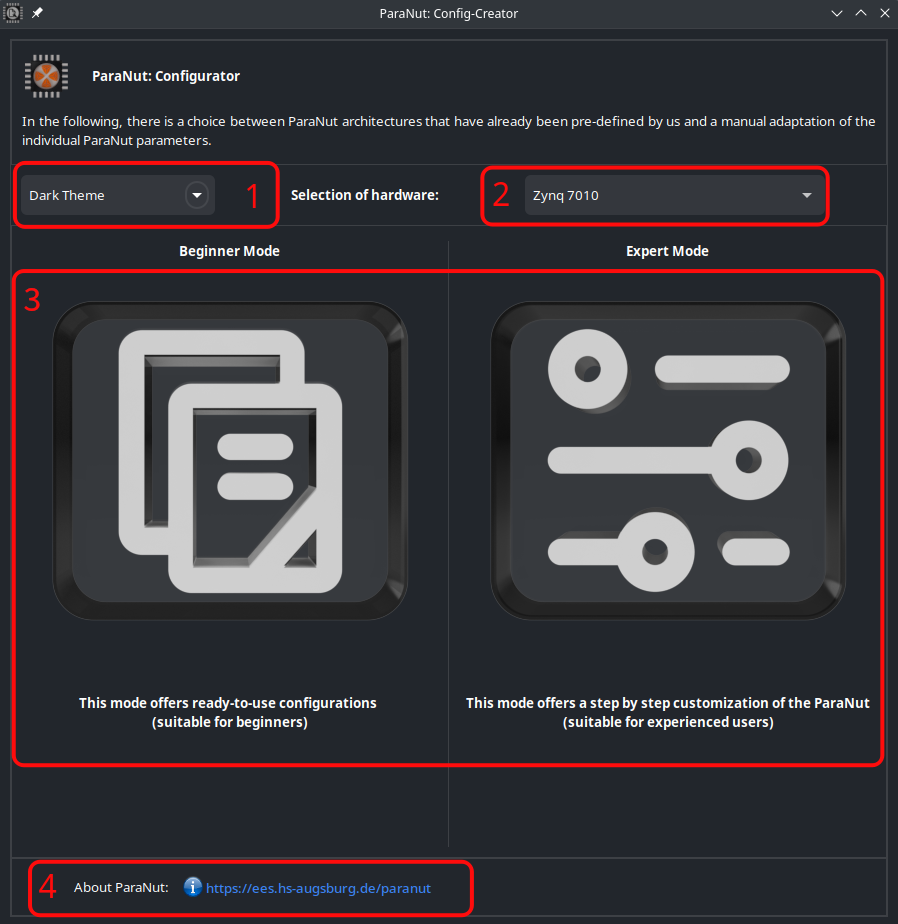
\includegraphics[width=15cm]{images/start_page}
        \par\end{centering}
    \caption{Screenshot of the starting page}
\end{figure}

\begin{enumerate}
	\item Select desired theme. You can choose between light and dark theme.
	\item Select your desired hardware to continue with the configuration progress.
	\item Choose between predefined configurations and a manual configuration of the ParaNut.
Beginner mode:
Contains a list of already \glqq ready-to-use\grqq{} configurations and your saved presets.
Expert mode:
Contains a step by step configuration process, where every module can be adjusted by certain parameters.
	\item These are links leading to an overview article of the ParaNut project from the embedded world exposition in 2020 and to the EES-ParaNut project GitHub.
\end{enumerate}

\newpage
\section{Beginner mode}

\begin{figure}[!h]
    \noindent \begin{centering}
        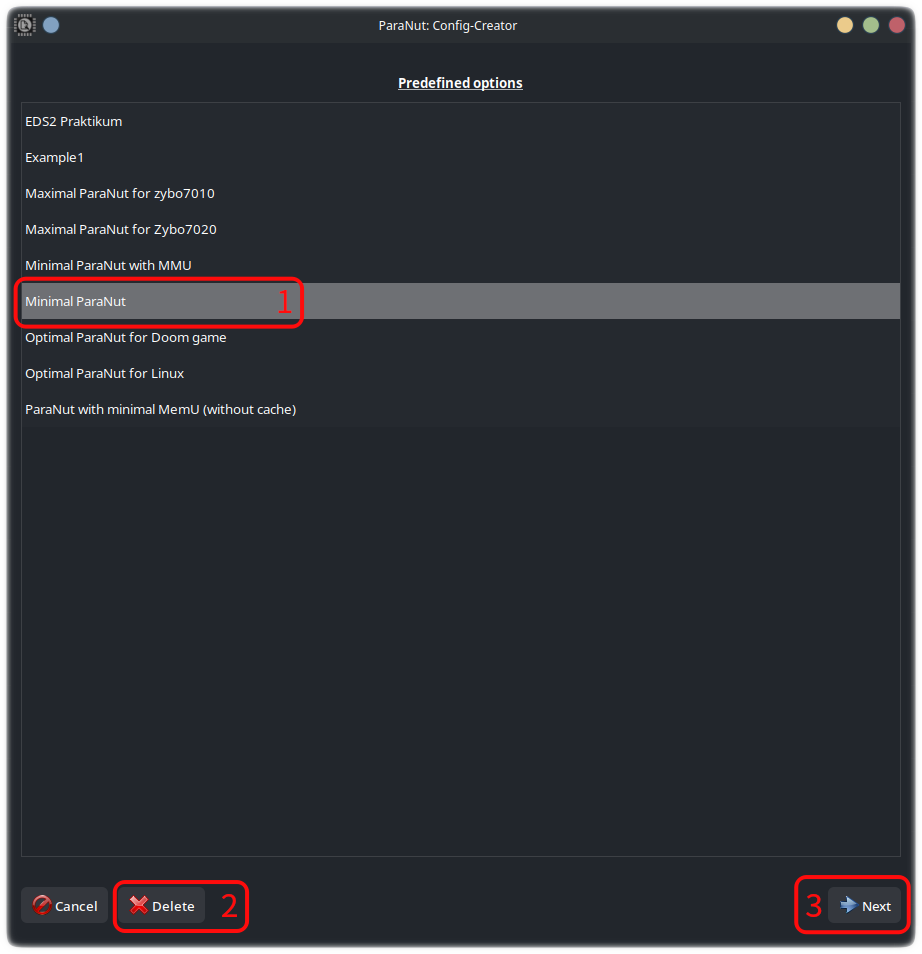
\includegraphics[width=15cm]{images/auto_page}
        \par\end{centering}
    \caption{Screenshot of the beginner mode page}
\end{figure}

\begin{enumerate}
	\item Each section represents either a predefined system or one of your saved presets. 
	\item Pressing the \glqq Cancel\grqq{}  button will redirect you to the starting page.

\end{enumerate}
\newpage
\section{Expert mode}

\begin{figure}[!h]
    \noindent \begin{centering}
        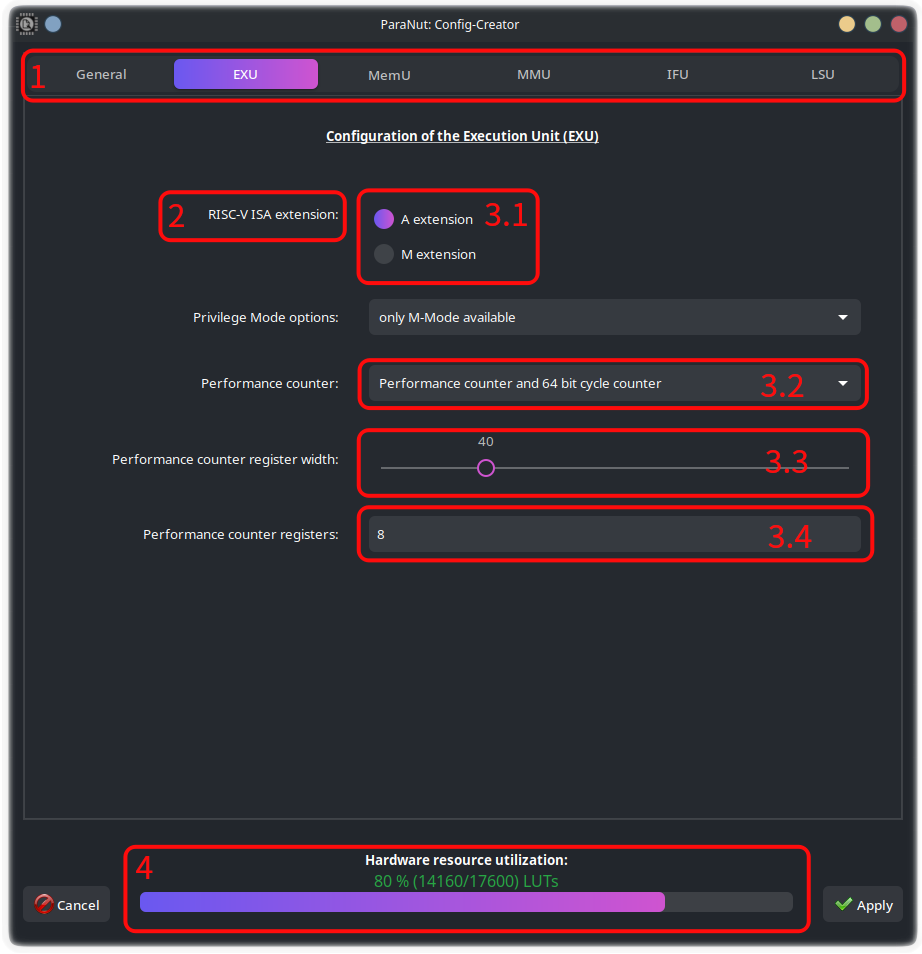
\includegraphics[width=15cm]{images/edit_page}
        \par\end{centering}
    \caption{Screenshot of the expert mode page}
\end{figure}

\begin{enumerate}
	\item The manual configuration page has a navigation bar, which is used to jump between the individual modules.
	\item Each module has its own parameters which reveal tips and explanations when hovering over them.
	\item The configuration process consists of three different input types:

	\begin{enumerate}
		\item[1] Checkboxes, which decide whether content should be added.
		\item[2] Comboboxes, which have drop-downs containing the different options to choose from.
		\item[3] Slider, which allows to select an accurate value.
		\item[4] Simple integer entries, resembling the desired value of the associated parameter.
  (invalid entries will return warnings or errors.)
	\end{enumerate}
	\item The hardware resource utilization progress bar resembles the used hardware resource capacity relative to its maximum resources.

		Pressing the \glqq Apply \grqq{} button will commit your entered values, while jumping to the overview page.
		Pressing the \glqq Cancel \grqq{} button will terminate the manual configuration process and you will be sent to the starting page.

\end{enumerate}
\newpage
\section{Overview page}

This page is the last stop before the finished configuration file. On this page all your manually selected or predefined options will be summarized, giving you the chance to make changes.

\begin{figure}[!h]
    \noindent \begin{centering}
        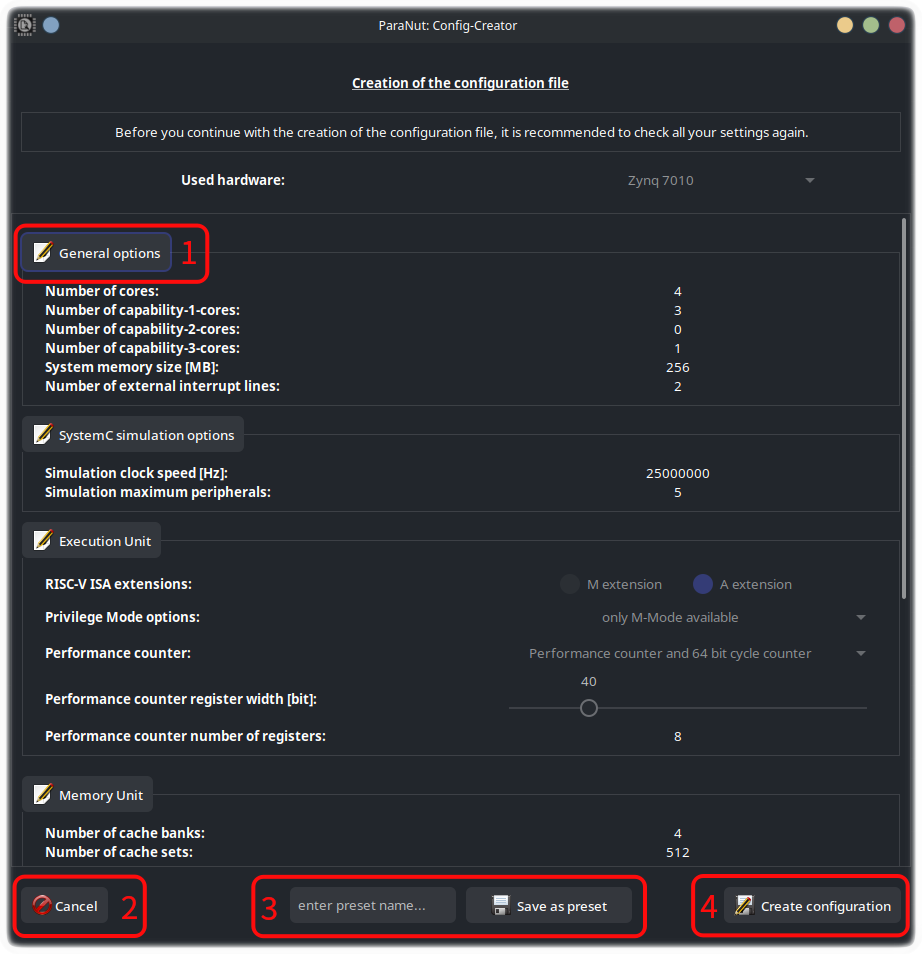
\includegraphics[width=15cm]{images/final_page}
        \par\end{centering}
    \caption{Screenshot of the overview page}
\end{figure}

\begin{enumerate}
	\item Each different module has ist own section with an \glqq Edit\grqq{}  button, which leads to the corresponding module page in the manual configuration.
	\item The \glqq Cancel\grqq{}  button will lead you back to the starting page.
	\item Your configuration will be saved as a preset. From now on it will be shown in your Beginner mode section of the tool.
	\item Your configuration will be saved as a finished config.mk file on your computer.

\end{enumerate}

\end{document}
